\documentclass[11pt, singlecolumn, citestyle=authoryear]{elegantbook}
\definecolor{customcolor}{RGB}{153,204,255}
\colorlet{coverlinecolor}{customcolor}
\usepackage{wrapfig}
\usepackage{lmodern}
\usepackage{lipsum,graphicx}
\usepackage[utf8]{inputenc} %unicode support
\usepackage[T1]{fontenc}


\newcommand{\compresslist}{%
	\setlength{\itemsep}{0pt}%
	\setlength{\parskip}{1pt}%
	\setlength{\parsep}{0pt}%
}


\title{FUTURE-DATA\\Dublin Bikes}
\date{Due: April 21, 2023}
\author{Ariana Alves Antunes, Imelda Finn, Marcus Ò Faolain}

\begin{document}
	\mainmatter 
	
\chapter*{FUTURE-DATA\\Dublin Bikes \\\ Ariana Alves Antunes, Imelda Finn, Ó Faoláin}

 	\section*{Introduction}
This assignment is measuring the impact of pandemic on Dublin City Bikes within different scenario. 
	

\section{The impact of the pandemic on bike usage}
%To assess the impact of the pandemic on the city-bike usage;
	Due to lockdowns and restrictions in Dublin during COVID,  bike usage was directly impacted as shown in the figures below from 2019 and 2020, with more people  choosing to cycle over public transportation.  However with businesses closed and people working from home, the usage dropped by half. Just Eat Dublin Bikes’ latest summary statistics below as at 31/08/2019, current valid annual subscribers was 66,940 with €25 membership fee, plus revenue made with advertising. 

	\begin{figure}[h!]
		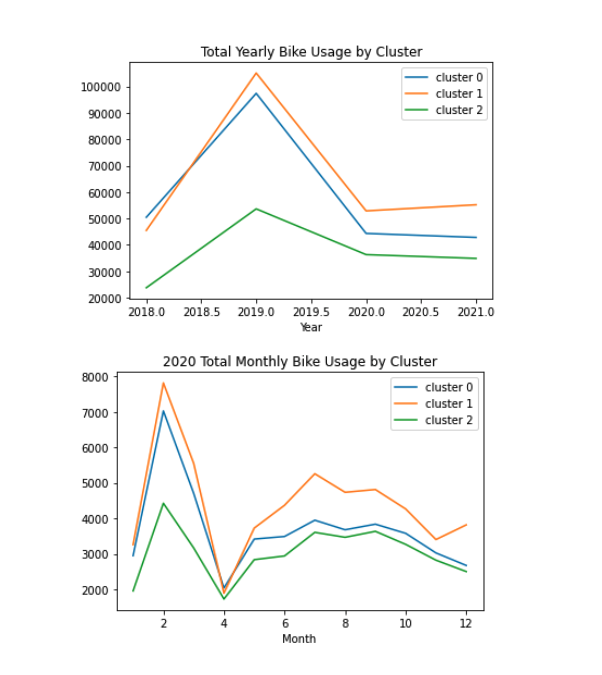
\includegraphics[width=0.7\textwidth]{../graphs/usaged_total_plus2020.png}
		\caption{Total bike usage and total usage for 2020}
		\label{fig:surface}\label{fig:model}
	\end{figure}

As can be observed from the graphs the contrast between before the pandemic started and 4 months after, there is a decline between full lockdown and when restrictions imposed by the Government were lifted. Since the bikes are membership payments on a yearly basis, the risk of not acquiring new clients could be a major risk for the business, still the essential works were a big part of the new audience being attracted to Dublin bikes. 

\begin{table}[h!]
	\begin{tabular}{|l|r|r|}
		Year & Usage \\
		2018 & 13464.0 \\
		2019 & 26501.0 \\ 
		2020 & 11106.0 \\ 
		2021 & 8188.0 \\ 
		
	\end{tabular} 
\end{table}



\section{Predicted bike usage for 2020}
%2. To estimate how the city-bike usage would have been without the pandemic (e.g., 2020) 

Bike usage was way down compared to the prediction.\footnote{RidgeCV(alphas=(0.1, 1.0, 10.0), cv=None, fit\_intercept=True, gcv\_mode=None, normalize=False, scoring=None, store\_cv\_values=False)}  
The prediction isn't too bad for January, February, but usage drops at the end of February and stays down for the rest of the year.
\begin{figure}[!htbp]
	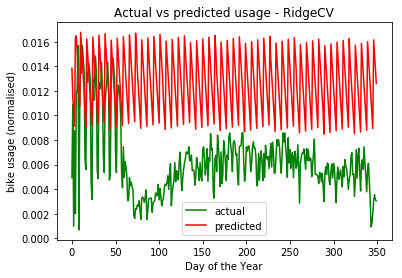
\includegraphics[width=0.7\textwidth]{../graphs/pred_2020.png}
	\caption{Predicted bike usage in 2020, compared to actual usage}
	\label{fig:surface}
\end{figure}

The pandemic also led to changes in cycling infrastructure in Dublin. The Dublin City Council implemented temporary measures, such as pop-up bike lanes and widened footpaths, to support cycling and promote social distancing. These measures were later made permanent, resulting in an increase in the number of dedicated cycle lanes across the city.

Overall, the pandemic  has presented an opportunity for bike usage in Dublin, with more people choosing to cycle as a means of transport. The increased interest in cycling has led to improvements in cycling infrastructure and the creation of more cycling-friendly routes in the city.


	
\section{Technical/Data issues}
We excluded stations with less than 300,000 data points.   None of the stations were open the whole time. The variable modelled is usage, which is the absolute difference in available bikes from one time point to the next.  For modelling, this is normalised by dividing by the number of bike stands.

There was some missing data for a few days in June and December 2019 and in January 2020.  This appears to be a system-wide issue.  The data usage calculation (diff) was re-started after each discontinuity, so a data-point was dropped for each one.

Each cluster contains 2 stations, as per the table below.   The clusters were identified by analysing pre-pandemic usage. Cluster 2 stations had similar pre-pandemic characteristics and both serve hospitals. 



	
\begin{table}[h]
	\begin{center}
	\begin{tabular}{lrrr}
		Station Name & cluster & bike stands\\
		FITZWILLIAM SQUARE EAST & 0 & 40 & blue\\
		HANOVER QUAY & 0 & 40 & blue\\
		NEW CENTRAL BANK & 1 & 40  & red\\
		YORK STREET EAST & 1 & 32  & red\\
		PARNELL SQUARE NORTH & 2 & 20 & green\\
		MATER HOSPITAL & 2 & 40 & green\\
		\label{tbl:stations}
	\end{tabular} 
\end{center}
\end{table}

\begin{figure}[h!]
	\begin{center}
	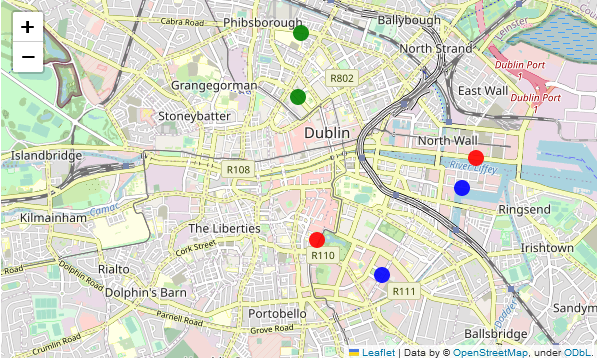
\includegraphics[width=0.5\textwidth]{../graphs/bikeStationMap.png}
	\caption{Selected Bike Stations}
	\label{fig:stations}
\end{center}

\end{figure}
\section*{Code Reference}
\texttt{https://github.com/Arianaxsz/ML-Project}

Code in \texttt{project\_group\_2.ipynb}, \texttt{py/project\_group\_2.py}

\texttt{Pre-processing: code/dublin\_bike\_analysis.ipynb}

\texttt{Model: code/model\_q2.ipynb}

\texttt{Data Visualization: code/Usage graphs.ipynb}

%===============================================================

% # Code snippets

%\vspace{.25cm}
%\noindent  %\href{https://www.researchgate.net/profile/Adam_Przeworski/publication/240357392_Classifying_Political_Regimes/links/0deec532194849aefa000000/Classifying-Political-Regimes.pdf}{Alvarez, Cheibub, Limongi, and Przeworski (1996)}




\end{document}
